\documentclass[a4paper,10pt]{article}
%\usepackage[utf8]{inputenc}
\usepackage{graphicx}
\usepackage{subcaption}
\usepackage{parskip}
\usepackage{amsmath}
\usepackage{listings}
\usepackage{color}
\usepackage{listings}

\definecolor{red}{rgb}{1,0,0}
\definecolor{green}{rgb}{0,1,0}
\definecolor{codegreen}{rgb}{0,0.6,0}
\definecolor{codegray}{rgb}{0.5,0.5,0.5}
\definecolor{codepurple}{rgb}{0.58,0,0.82}
\definecolor{backcolour}{rgb}{0.95,0.95,0.92}

\lstdefinestyle{mystyle}{
    backgroundcolor=\color{backcolour},   
    commentstyle=\color{blue},
    numberstyle=\tiny\color{codepurple},
    stringstyle=\color{codegreen},
    basicstyle=\footnotesize,
    breakatwhitespace=false,         
    breaklines=true,                 
    captionpos=b,                    
    keepspaces=true,                 
    numbers=left,                    
    numbersep=5pt,                  
    showspaces=false,                
    showstringspaces=false,
    showtabs=false,                  
    tabsize=2
}
 
\lstset{style=mystyle,language = Python}

%opening
\title{Assignments UNIK/TEK4660 Spring 2018}
\author{Joseph Knutson}

\begin{document}

\maketitle

\section*{Runge Kutta and the Lorentz Attractor}

Let ($r_1,r_2,r_3$) = (x,y,z) and $dx/dt = x^{(1)}$ consider the Lorentz system
\begin{align}
 x^{(1)} &= \sigma(y - x) \label{x} \\ 
 y^{(1)} &= x(\rho - z) - y   \label{y}\\
 z^{(1)} &= xy - \beta z  \label{z}
\end{align}
our job is to integrate these velocities in order to create the pathline $l(x,y,z)$.
This can be done in a simple manner, using the forward euler algorithm, or in a more accurate manner user the 4th order runge kutta algorithm.

\subsection*{Forward Euler}

Solved numerically with forward Euler, the e.o.m.(s) will look like this:
\begin{align}
 x_{t+h} &= \sigma(y_{t} - x_{t})*h + O(h^2) \\
 y_{t+h} &= \left[x_{t}(\rho - z_{t}) - y_{t}\right]*h + O(h^2)\\
 z_{t+h} &= (x_{t}y_{t} - \beta z_{t})*h + O(h^2)
\end{align}
where $t\ +\ h$ is a timestep forward (into the future), $t$ is the current time and $O(h^2)$ is the size of the error.

For the Lorentz attractor, $\rho = 28,\ \sigma = 10$ and $\beta = 8/3$. 
Implementing this solution in python over 10 time units using forward euler and $x_0 = 10,\ z_0 = 10,\ z_0 = 10,$ returns the graph in figure \ref{1}


\begin{figure}
 \centering
 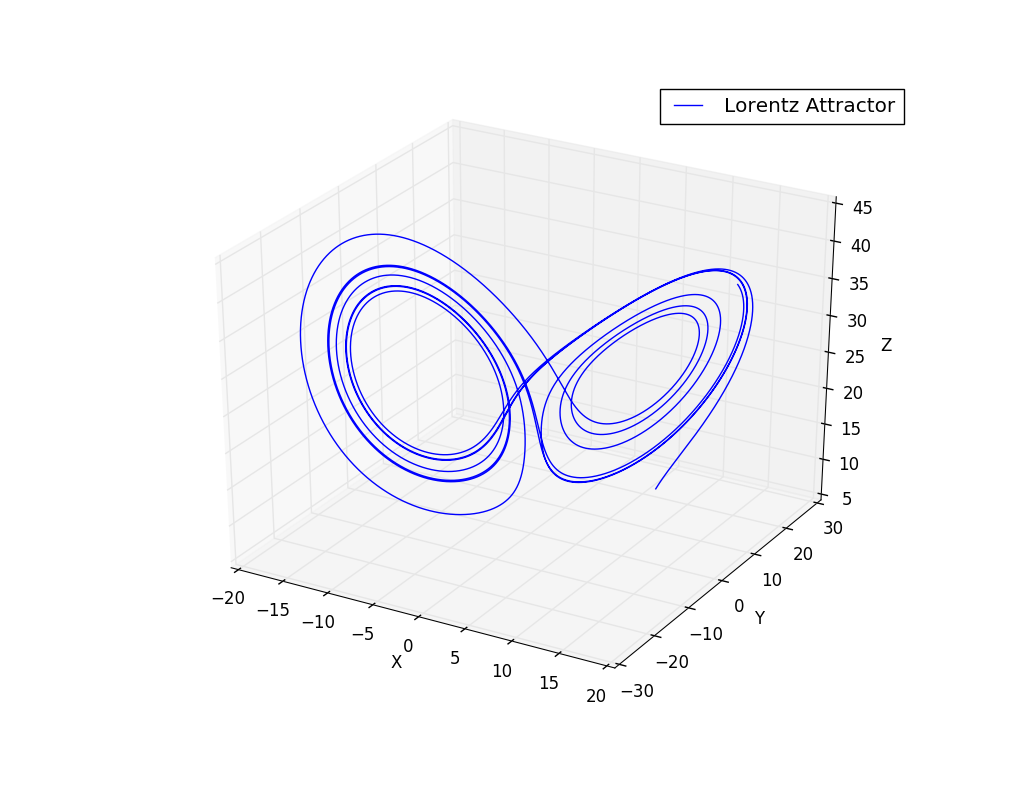
\includegraphics[width = \linewidth]{euler}
 \caption{Lorentz attractor made in Python using the forward Euler algorithm.}
 \label{1}
\end{figure}

\clearpage

\subsection*{RK4}
Instead of implementing Runge-Kutta 4, we use a python module (scipy).
%          &= \sigma y(y - x) + x(x(\rho - z) - y) - \beta (xy - \beta z)̇ \nonumber\\
%          &= \sigma y^2 - \sigma yx + \rho x^2 - x^2 z -xy - \beta xy + \beta^2 z 
%          &= \sigma(y - x)(\rho - (xy - \beta z )) - (x(\rho - z) - y) \nonumber\\
%          &= \sigma \rho (y-x) - \sigma xy(y-x) + \sigma \beta (y-x)z - x\rho + xz + y  \nonumber  \\
%          &=  \sigma \rho y- \sigma \rho x - \sigma xy^2 -\sigma x^2y \nonumber\\ 
%          &+ \sigma \beta yz- \sigma \beta xz - x\rho + xz + y   \label{y2}\\
% 	 &= \sigma((x(\rho - z) - y) - (\sigma(y - x))) \nonumber  \\
%          &= \sigma \rho x - \sigma  x z - \sigma y - \sigma^2y + \sigma^2 x  \label{x2}  \\

% 	 &=   \sigma((\ref{y2}) - (\ref{x2})) \texttt{    (equation labels)}
% 	 & \nonumber \\
% 	 &= -2\sigma \rho x + \sigma  x z + \sigma y + \sigma^2y - \sigma^2 x   \nonumber \\
% 	 &+ \sigma \rho y - \sigma xy^2 -\sigma x^2y + \sigma \beta yz- \sigma \beta xz - x\rho + xz + y 
The scipy.integrate library has a method called ode which contains various integration methods, including rk45. The script I've implemented looks something like this:
\begin{lstlisting}
u0 = [10,10,10]             #Initial positions.

def f(t,u,sigma,rho,beta):  #Right hand side of -
    x,y,z = u               #differential equations.
    return [sigma*(y-x), x*(rho-z) - y, x*y-beta*z]

#initialize integrator with function f, "dopri5" is rk45
r1 = ode(f).set_integrator('dopri5',atol=1e-6)

#integrate with initial conditions
r1.set_initial_value(u0, 0).set_f_params(sigma,rho,beta) 
\end{lstlisting}

In figure \ref{2} and \ref{3} you can see both the rk45 solution of the Lorentz attractor and both solutions superimposed on eachother.
As you might be able to pick up from these figures, the euler solution is unable to stay on track due to it's increase in numeric error.

\begin{figure}
 \centering
 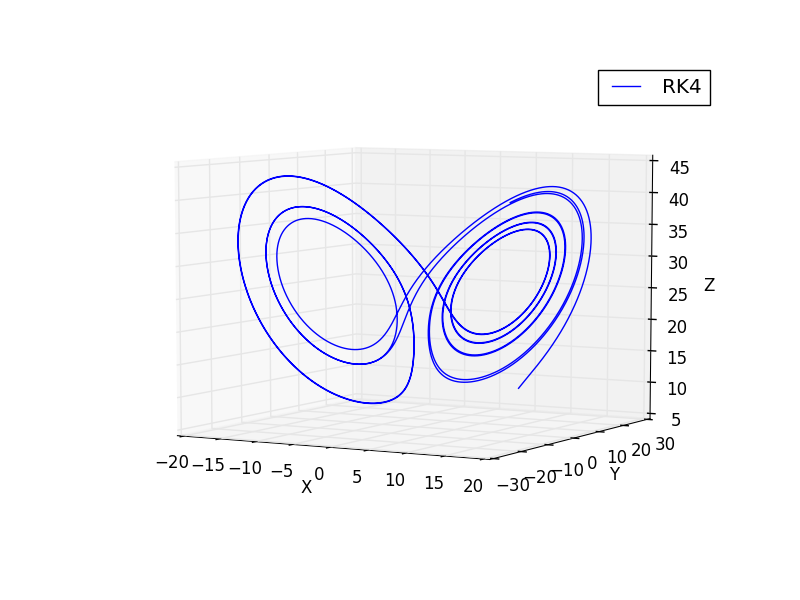
\includegraphics[width = \linewidth]{rk4}
 \caption{Lorentz attractor made in Python using the rk45 algorithm. The graph differs from the Euler solution in that the pathline stays on the same path, making the lines overlap more. The euler solution however seems to not overlap itself, making the lines more spread out.}
 \label{2}
\end{figure}

\begin{figure}
 \centering
 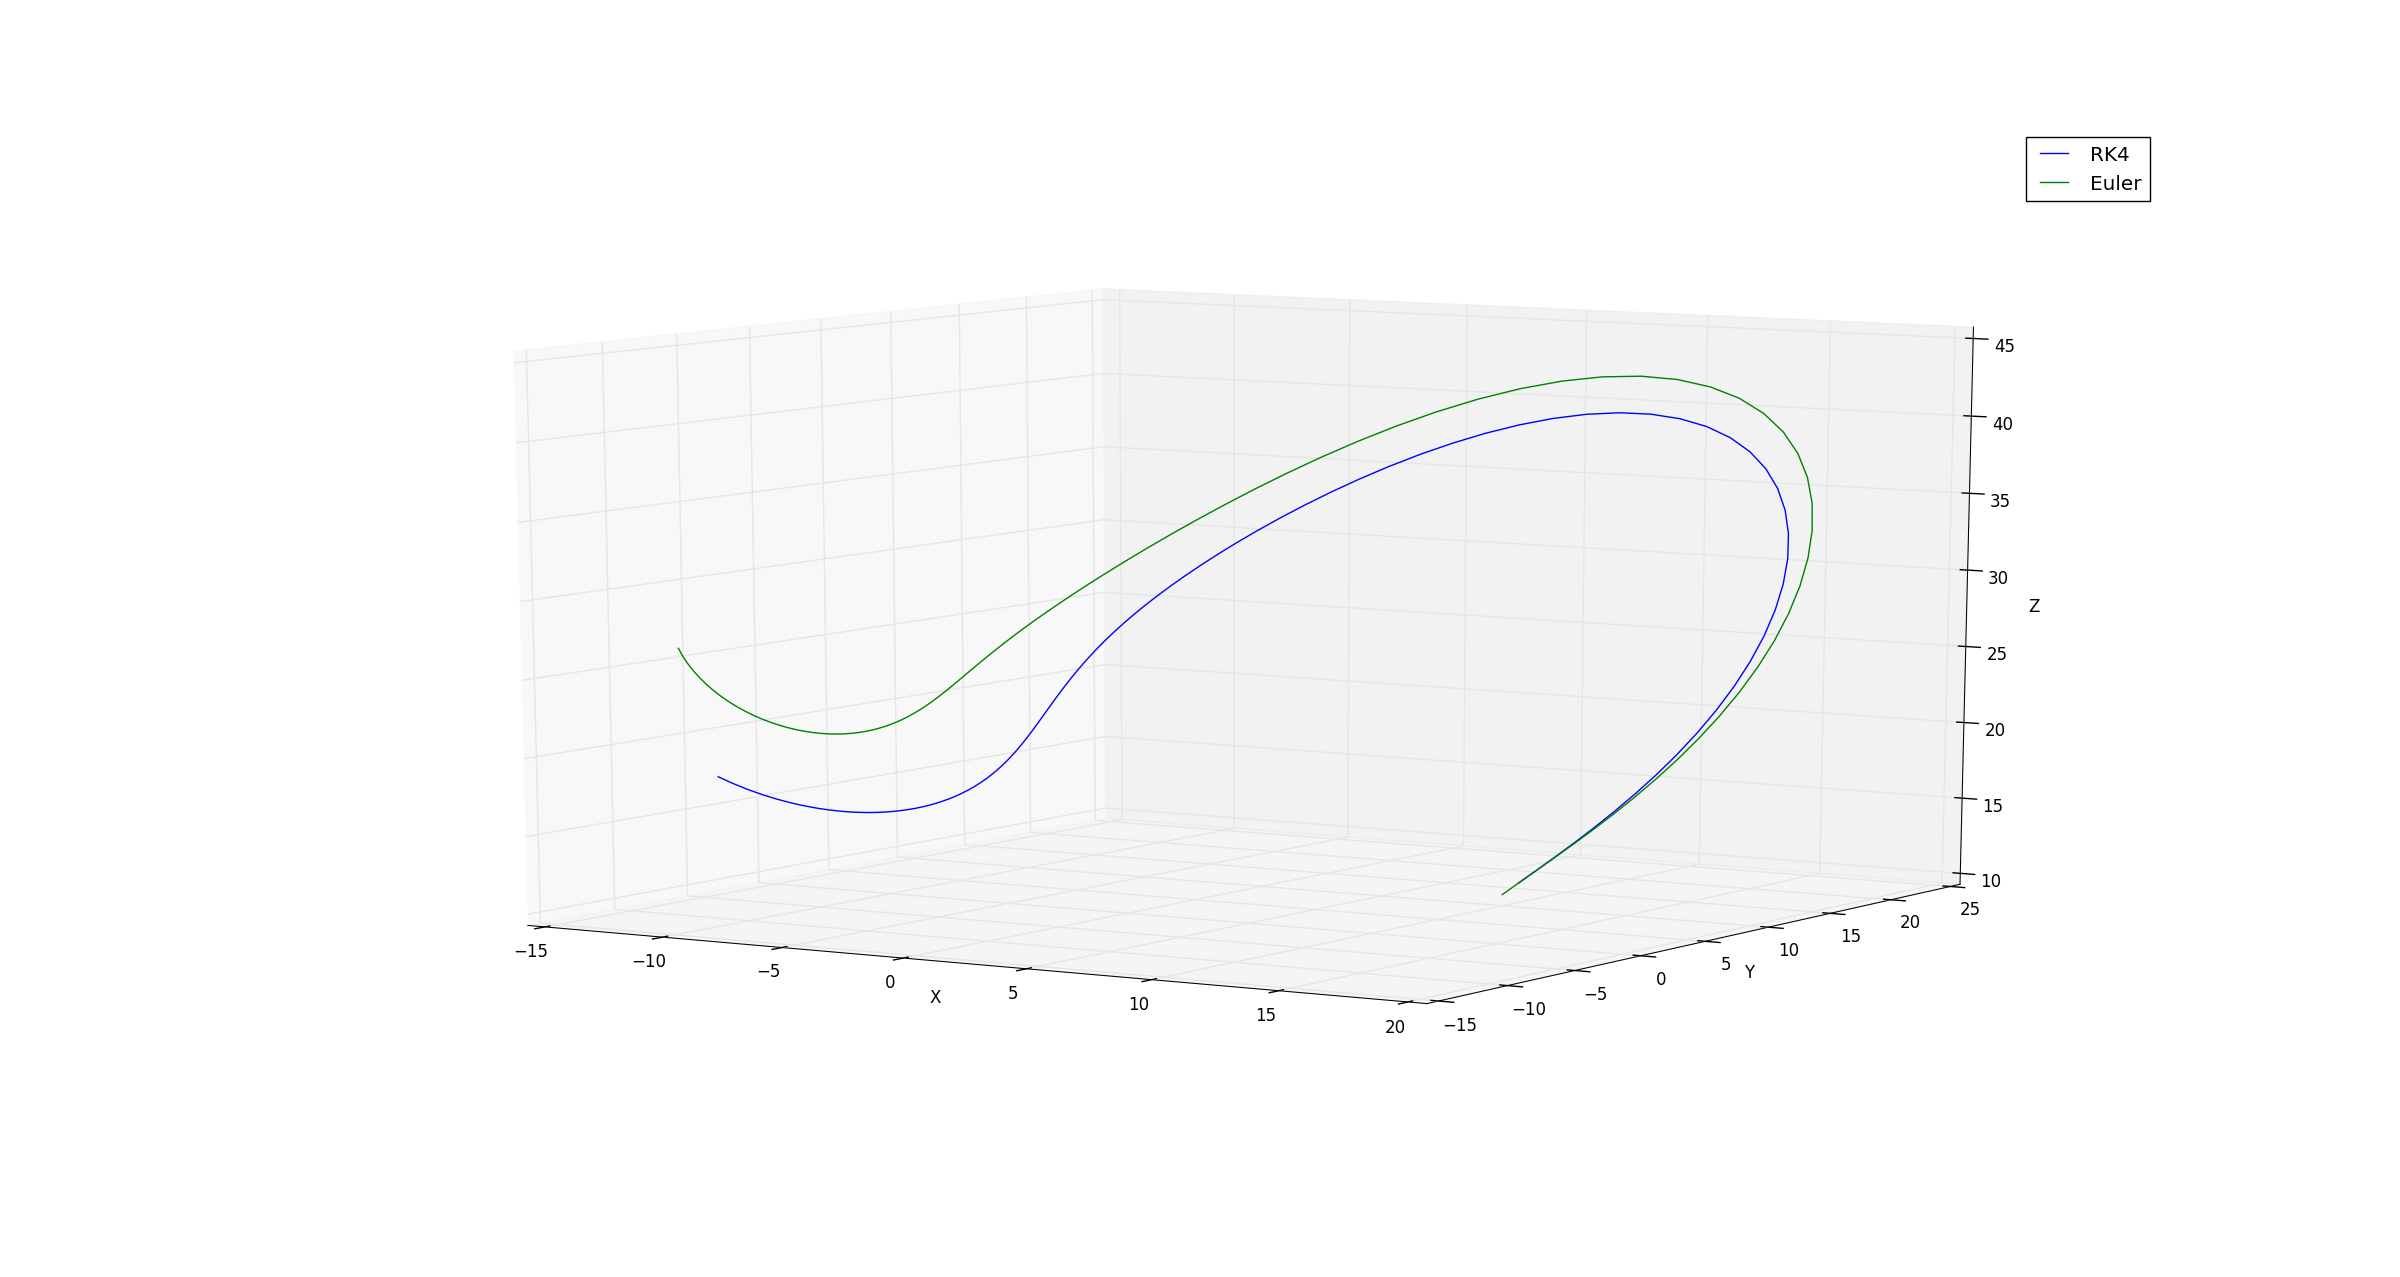
\includegraphics[width = \linewidth]{compare}
 \caption{Line segments of both solutions. Observe how the error in the euler solution drastically increases from the more accurate rk45 solution.}
 \label{3}
\end{figure}
\section*{Task A}
We now want to calculate $\kappa$ and  $\tau$, the curvature and torsion.
These are expressed in equation \ref{eq1} and \ref{eq2}:
\begin{equation}\label{eq1}
 \kappa = \frac{||\dot{r} \times \ddot r||}{||\dot r||^3}
\end{equation}
\begin{equation}\label{eq2}
 \tau = \frac{\dot{r} \cdot (\ddot r \times \dddot r)}{||\dot{r} \times \ddot r||^2}
\end{equation}
Instead of deriving these expressions and the derivatives analytically, let's simply find the 2nd and 3rd differentials numerically
Thanks to rk45/ode45, we now have $\vec r$. By using the differential equations we started with; \ref{x}, \ref{y} and \ref{z}, we possess the velocity, $\dot r$ too.
The expressions for the second derivatives can be found in equation \ref{x2}, \ref{y2} and \ref{z2}. 
\begin{align}
x^{(2)} &= \sigma(y^{(1)} - x^{(1)}) \label{x2}\\
         &\nonumber \\
 y^{(2)} &= x^{(1)}(\rho - z) - xz^{(1)} - y^{(1)} \label{y2} \\
         &\nonumber \\
 z^{(2)} &= x^{(1)}y + xy^{(1)} - \beta z^{(1)} \label{z2} 
\end{align}
You can see that the product rule has been used in both equation \ref{y2} and \ref{z2}. Repeating this differentiation gives us expressions for the third derivatives.
\begin{align}
x^{(3)} &= \sigma(y^{(2)} - x^{(2)}) \label{x3} 
\end{align}
\begin{align}
y^{(3)} &= x^{(2)}(\rho - z) - 2x^{(1)}z^{(1)} - xz^{(2)} - y^{(2)}
\end{align}
\begin{align}
z^{(3)} &= x^{(2)}y + 2x^{(1)}y^{(1)} + xy^{(2)} - \beta z^{(2)}
\end{align}
After acquiring x, y and z from the numerical integration, we can already begin implementing the code that gives us the derivatives:
\begin{lstlisting}
vx = sigma*(y-x) #derivatives from 1st to 3rd order
vy = x*(rho-z)-y
vz = x*y-beta*z
x_2 = sigma*(vy - vx) 
y_2 = vx*(rho - z) - x*vz - vy
z_2 = vx*y + x*vy - beta*vz
x_3 = sigma*(y_2 - x_2)
y_3 = x_2*(rho - z) - 2*vx*vz - x*z_2 - y_2
z_3 = x_2*y + 2*vx*vy + x*y_2 - beta*z_2

\end{lstlisting}
% fig = plt.figure() #plotting
% ax = fig.gca(projection='3d')
% ax.plot(x_3, y_3, z_3, label='3rd Derivative Plot'
We now possess the derivatives from 1st to 3rd order.
% The code above has been used to plot the first, second and third order derivatives in figure \ref{vel}, \ref{acc} and \ref{accc}.
% 
% \begin{figure}
%  \centering
%  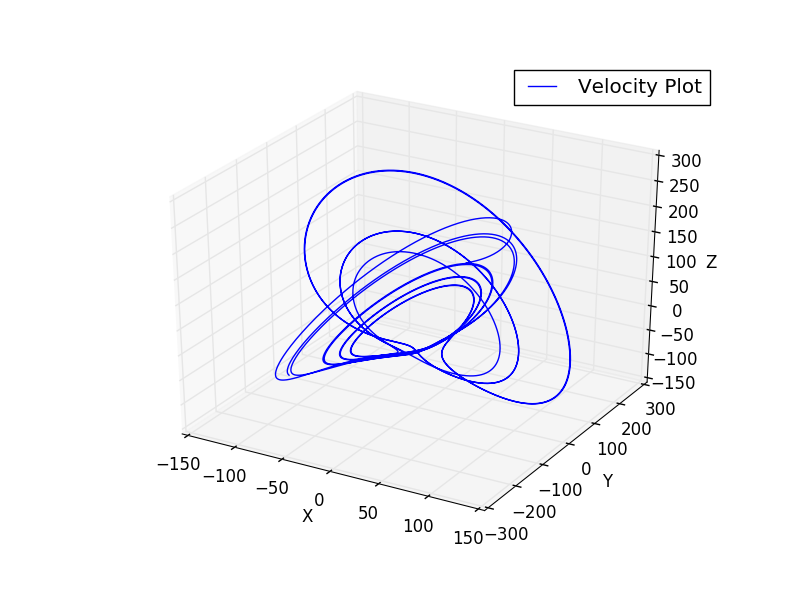
\includegraphics[width =0.5\linewidth]{vel}
%  \caption{1st order derivative of the Lorentz attractor, expressed with the initial differential equations in this paper. As a reminder, the initial conditions are $x_0 = y_0 = z_0 = 10$}
%  \label{vel}
% \end{figure}
% 
% \begin{figure}
% \begin{subfigure}{.5\textwidth}
% \centering
% 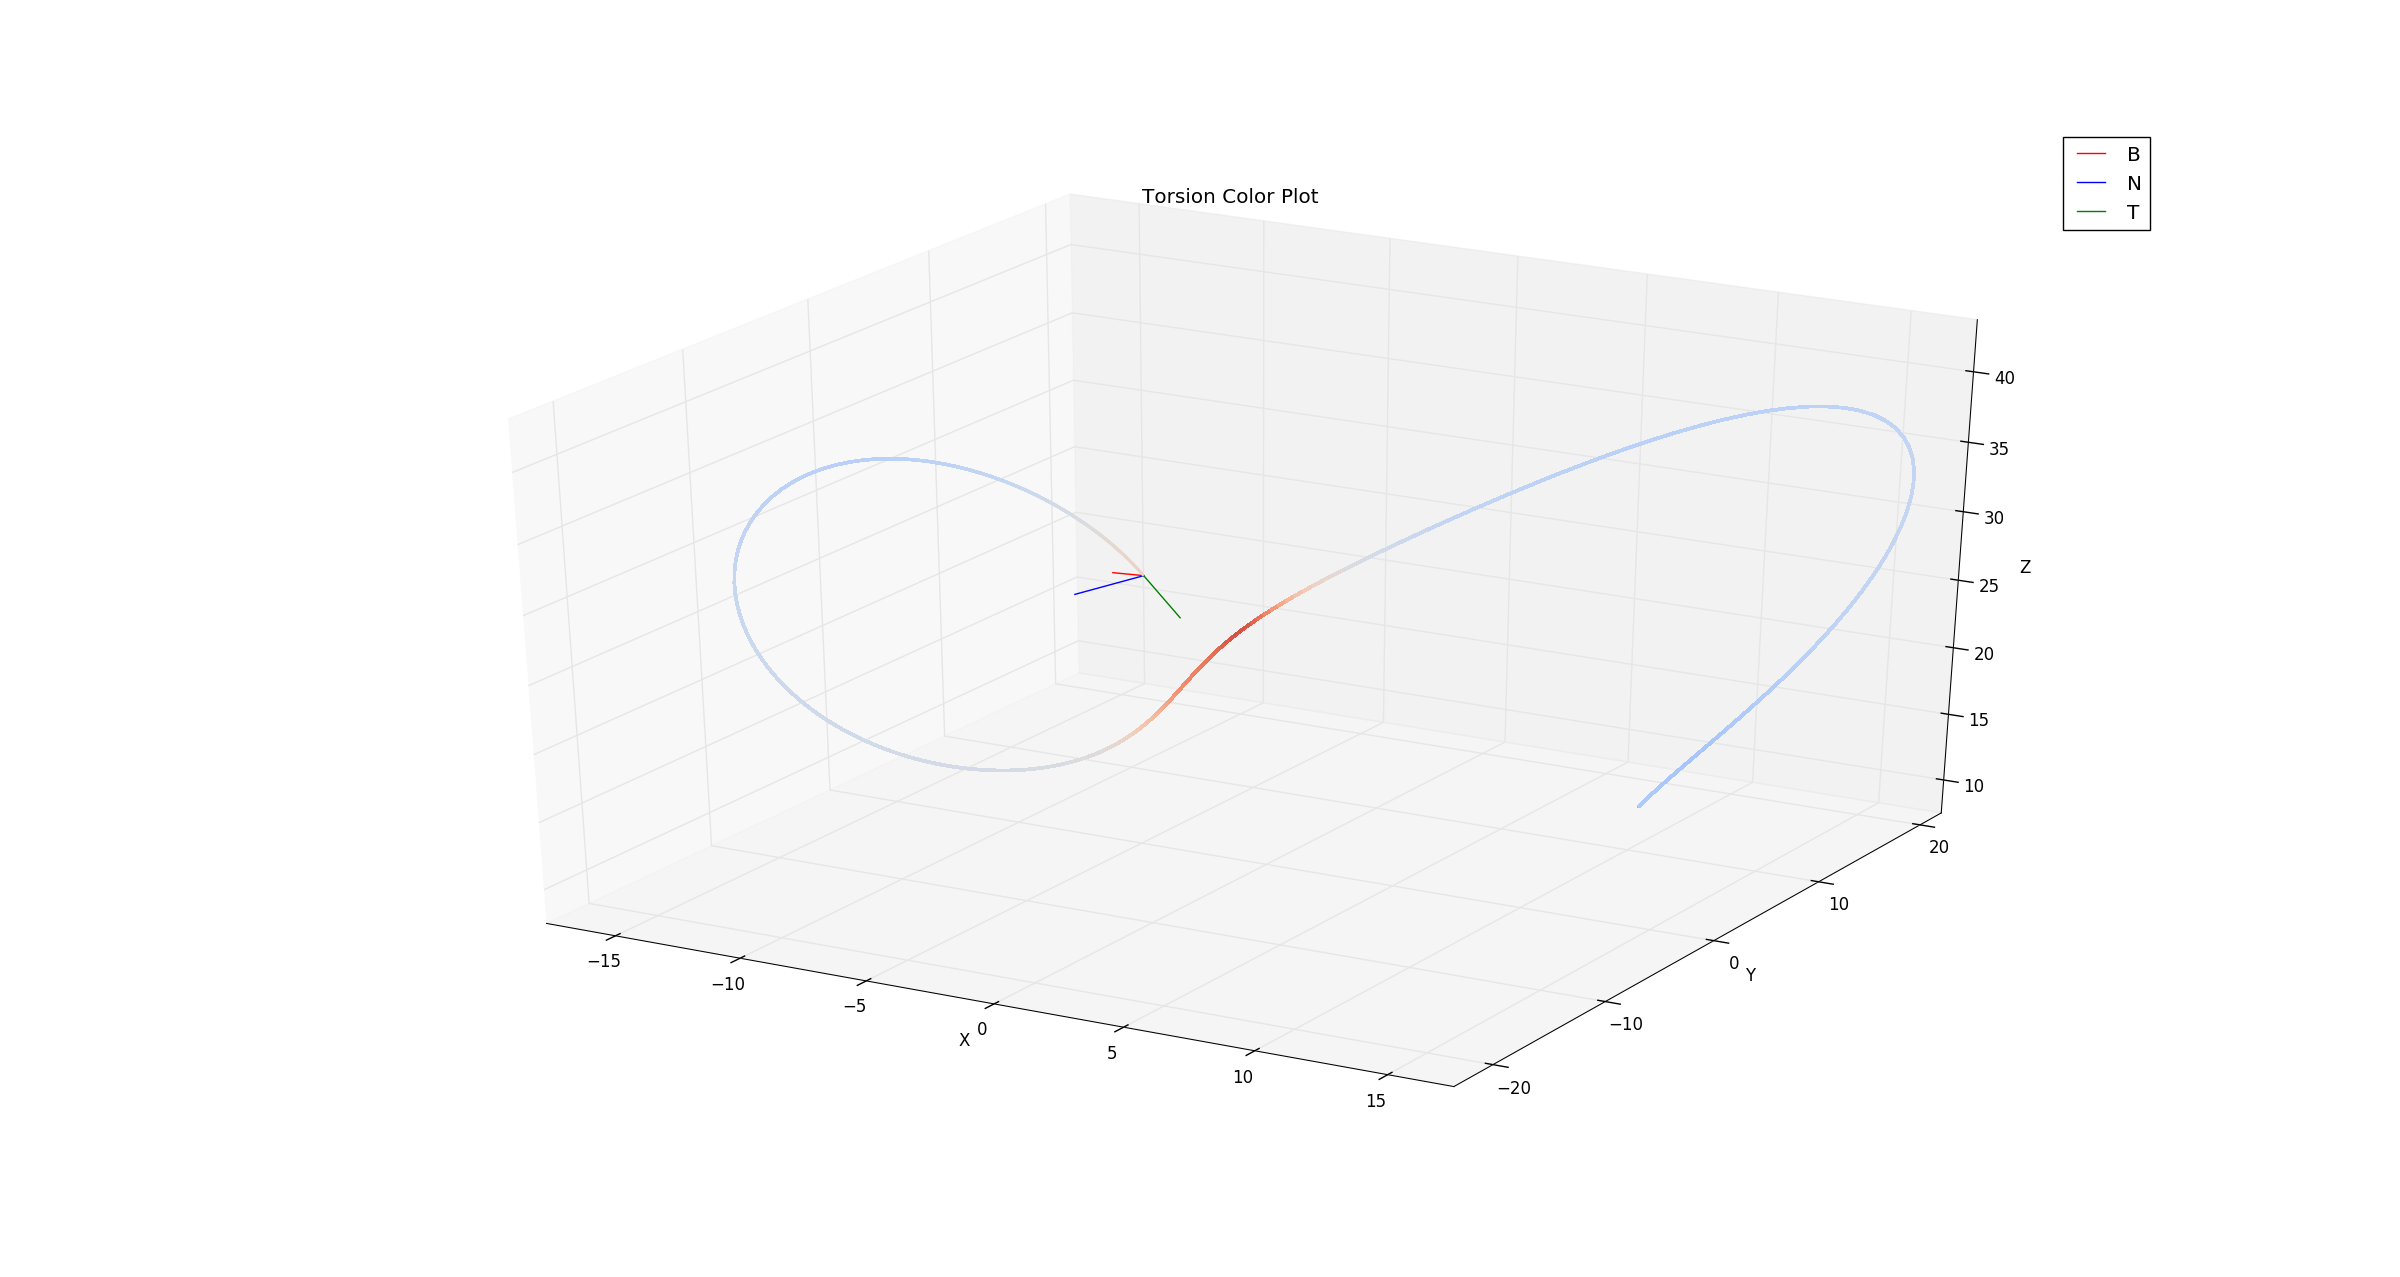
\includegraphics[width=1\linewidth]{2}
% \subcaption{2nd order derivative of the Lorentz attractor. Can be seen as the acceleration.}
% \label{acc}
% \end{subfigure}%
% \begin{subfigure}{.5\textwidth}
%  \centering
%  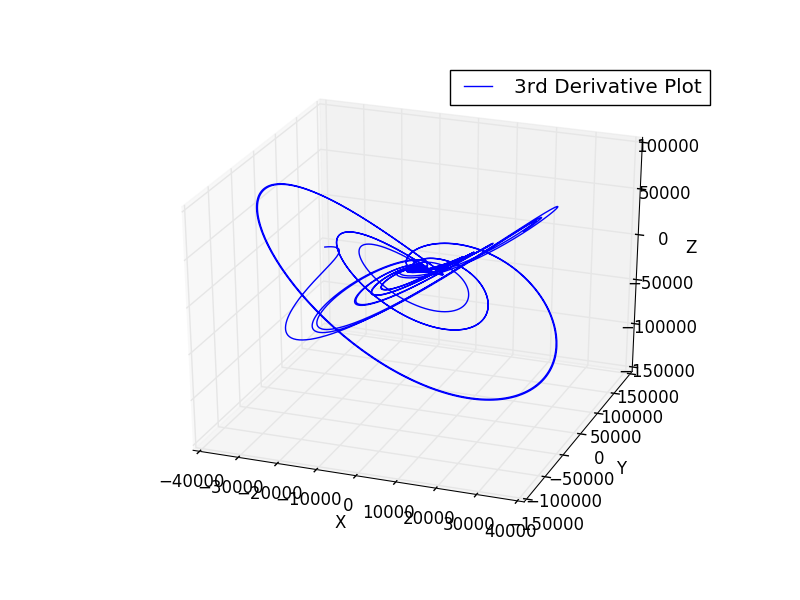
\includegraphics[width=1\linewidth]{3}
%   \subcaption{3rd order derivative of the Lorentz attractor.}
%   \label{accc}
%   \end{subfigure}
%  \caption{Derivatives of the Lorentz attractor. Notice the immense values of the third order derivative.}
% 
% \end{figure}


Using these expressions, we can immediately derive the curvature and torsion's values, based on equation \ref{eq1} and \ref{eq2}.
\begin{lstlisting}
curvature = np.zeros(n) #empty arrays
torsion   = np.zeros(n)
for i in range(n):
    #first we define the elements in the equations
    d  = np.asarray([ vx[i] ,vy[i] ,vz[i]]) #r dot
    dd = np.asarray([x_2[i],y_2[i],z_2[i]]) #r dotdot
    ddd = np.asarray([x_3[i],y_3[i],z_3[i]])#r dotdotdot
    dxdd = np.cross(d,dd)                   #rdot x rdotdot
    dnorm = np.linalg.norm(d)               #||rdot||
    dxddnorm = np.linalg.norm(dxdd)         #||rdot x rdotdot|| 
    
    curvature[i] = dxddnorm/(dnorm*dnorm*dnorm)
    torsion[i] = np.dot(d, np.cross(dd,ddd)) / (dxddnorm*dxddnorm)
\end{lstlisting}
Visualizing the Lorentz attractor while also visualizing the torsion and curvature can be tricky. Using color, line thickness and vectors could be viable.
Since these are scalar values, and I have no idea of how to vary line thickness, colorplots became the most optimal solution. In figure \ref{torso} and \ref{curv}, you can observe how the 
torsion and curvature behave along the attractor independently.
\begin{figure}
 \centering
 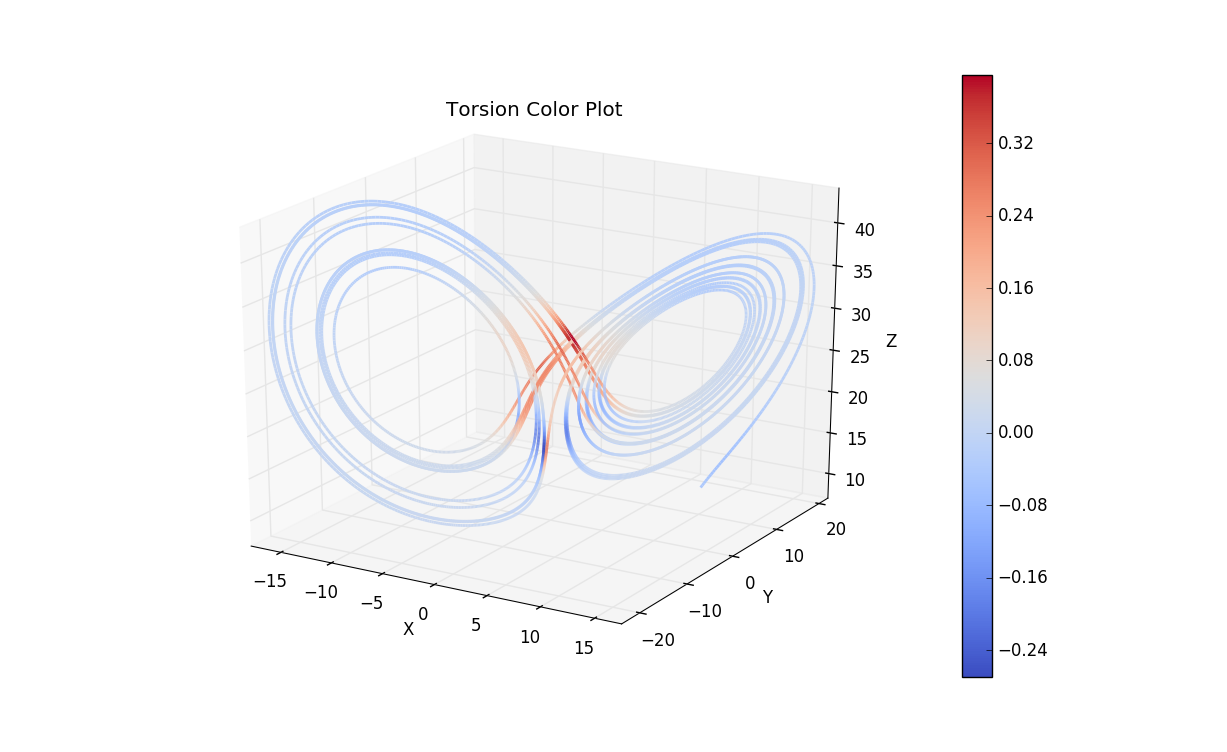
\includegraphics[width=\linewidth]{torso}
 \caption{Colorplot of the torsion along the Lorentz attractor. We can see that the most intense values happen during the transition from one spiral to another.}
  \label{torso}

\end{figure}
\begin{figure}
 \centering
 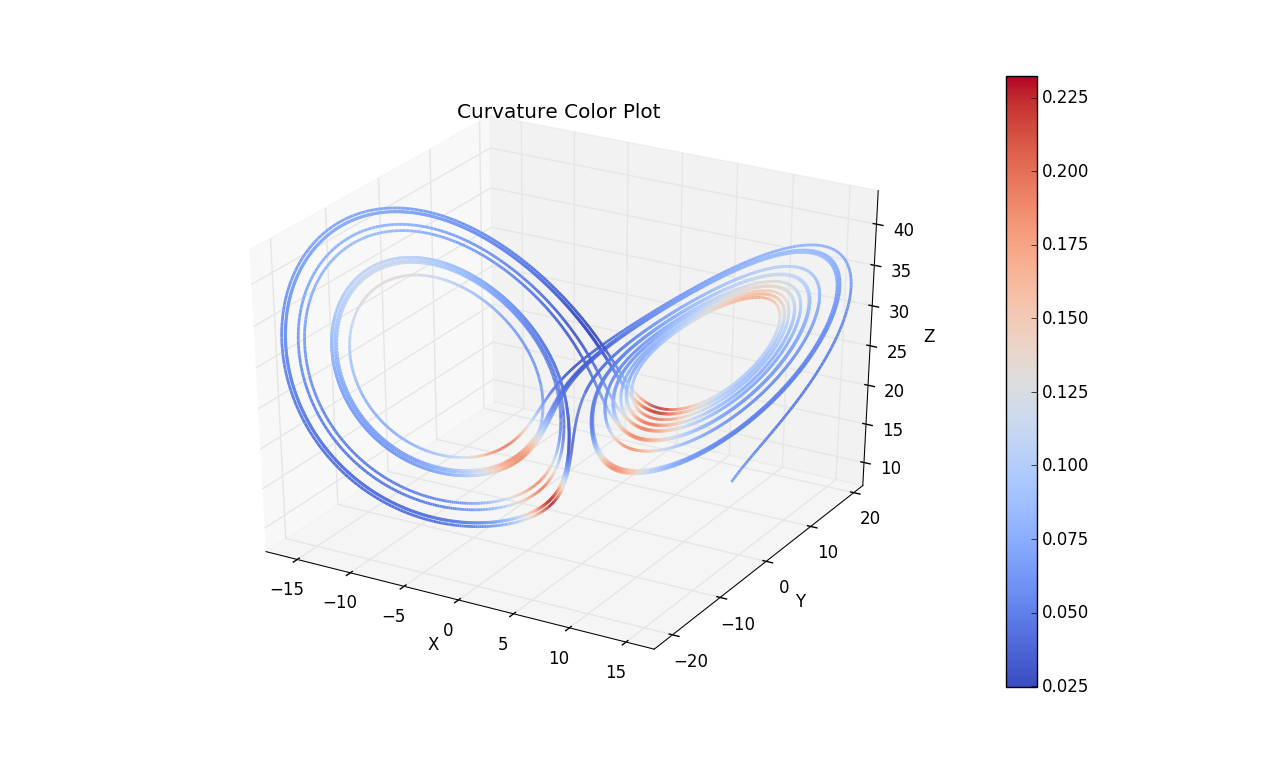
\includegraphics[width=\linewidth]{curv}
 \caption{Colorplot of the curvature. The maxima here seem to only happen at the "poles" of the spirals.}
  \label{curv}
  
\end{figure}
\clearpage
\section*{Task B}
Python was not suited for this task, but I made it. The tangent vector T, curve normal N and Binormal B are defined in the following equations:
\begin{align}
 T & = \frac{\dot r}{||\dot r ||} \\
 & \nonumber \\
 N & = \frac{\dot T}{||\dot T ||} \\
 & \nonumber \\
 B & = T \times N 
\end{align}
In order to find B, we need N and T. In order to find N we need T and in order to find T we need $\dot r$, which we already have! The code below implements these new vectors into our script:
\begin{lstlisting}
[...]
    T[:,i] = d[:]/dnorm       #dot r / norm(dot r)
    dT = (T[:,i]-T[:,i-1])/dt #dot T
    N[:,i] = dT/np.linalg.norm(dT)  #dot T/ norm(dot T)
    B[:,i] = np.cross(T[:,i],N[:,i])#T x B
\end{lstlisting}
Line 3 in the code above is a little cheat to find the derivative of T, $\dot T$. I first found the initial value of T($t_0$) and then subtracted it from T($t_0 + dt$) and divided by dt to find the derivative values repeadiately.
Now having the values, using them in the animation was unjustifyingly hard. Snapshots of the animation of both the torsion and curvature plots can be seen in figure \ref{mult1}, \ref{mult2}, \ref{mult3} and \ref{mult4}.

\begin{figure}
 \centering
 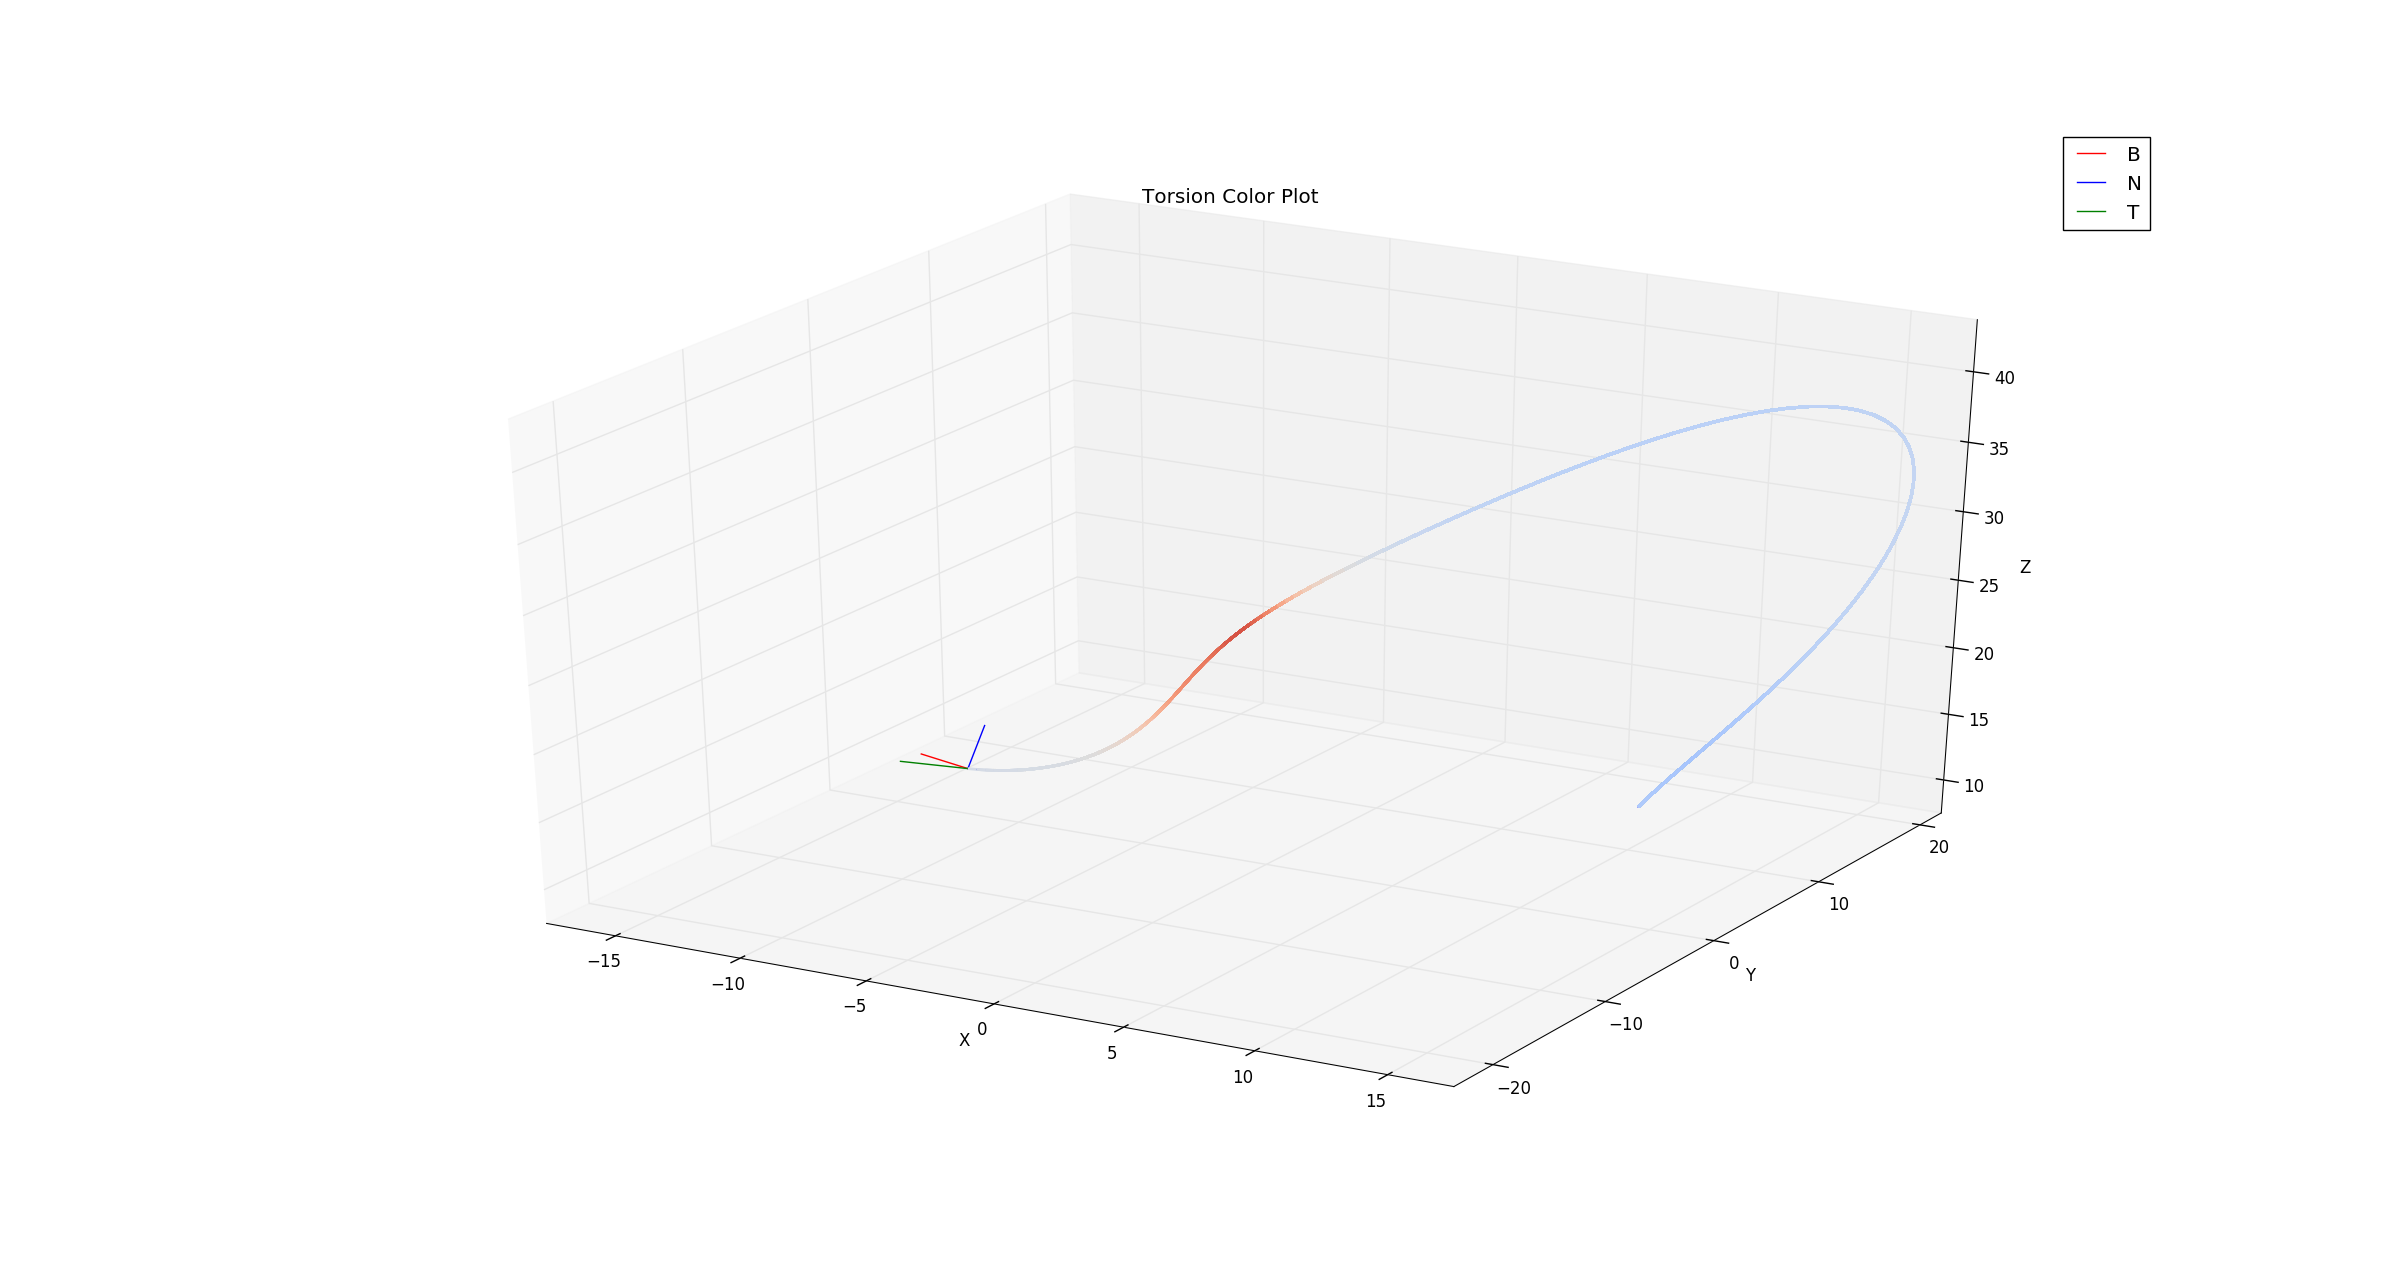
\includegraphics[width=\linewidth]{1}
 \caption{Torsion Animation with a live visualization of the T, N and B vectors. Sorry for the unreadable labels, R,G,B $=$ B,T,N}
  \label{mult1}  
\end{figure}

\begin{figure}
 \centering
 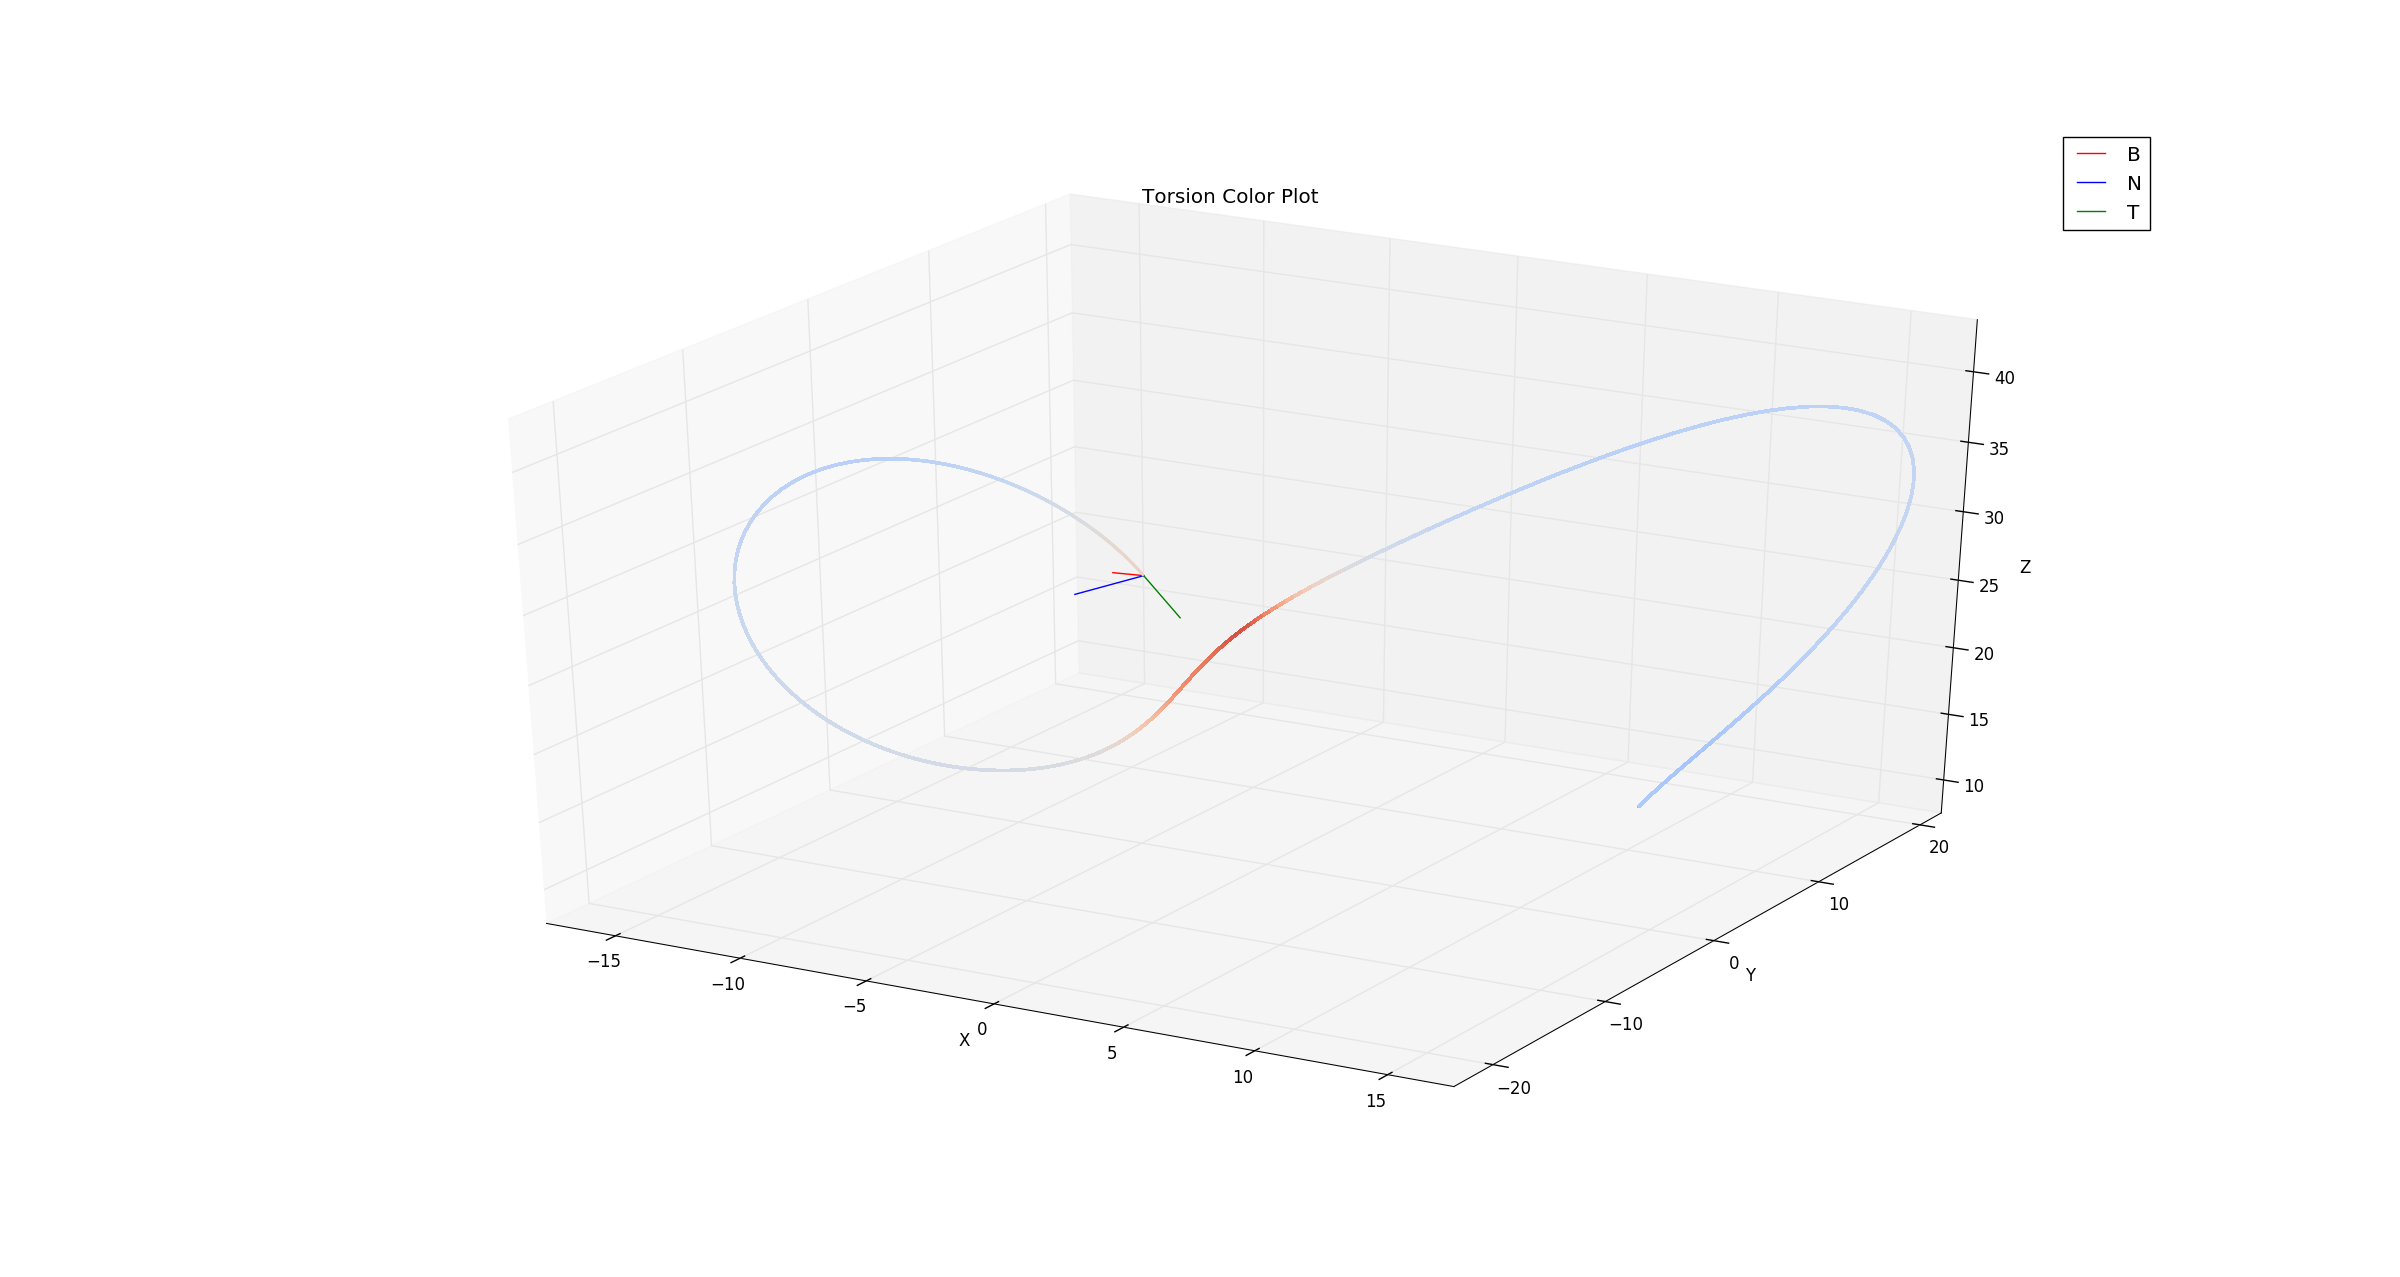
\includegraphics[width=\linewidth]{2}
 \caption{Torsion Animation few seconds later.}
  \label{mult2}
 \end{figure}
\begin{figure}
 \centering
 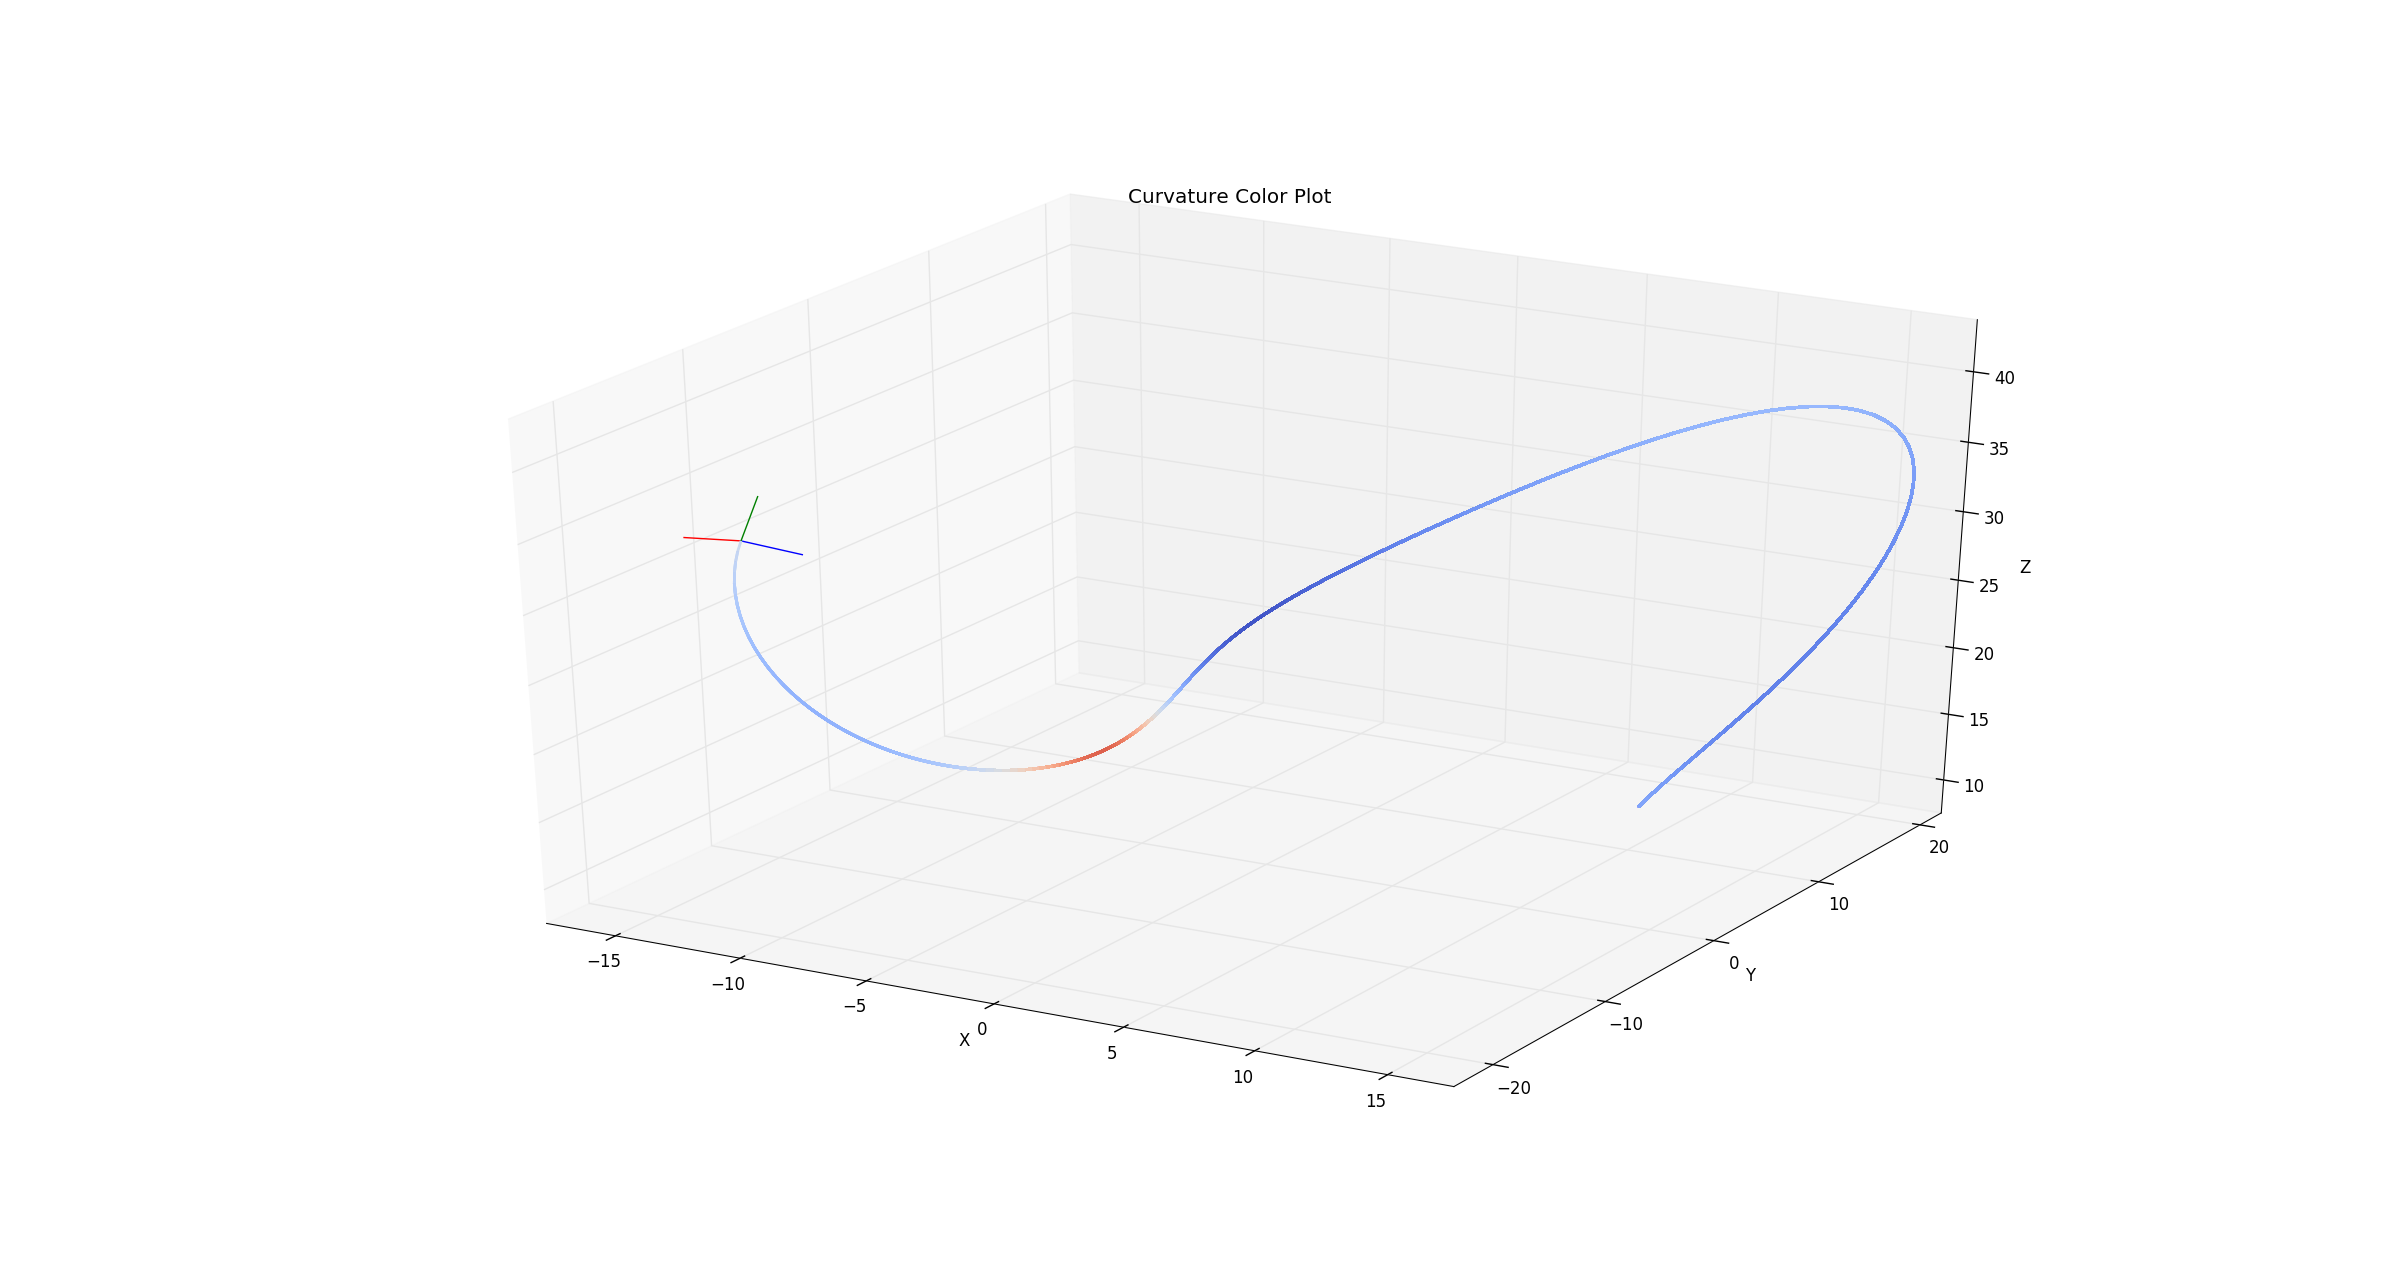
\includegraphics[width=\linewidth]{1c}
 \caption{Curvature Animation with a live visualization of the T, N and B vectors. RGB $=$ BTN }
  \label{mult3}  
\end{figure}

\begin{figure}
 \centering
 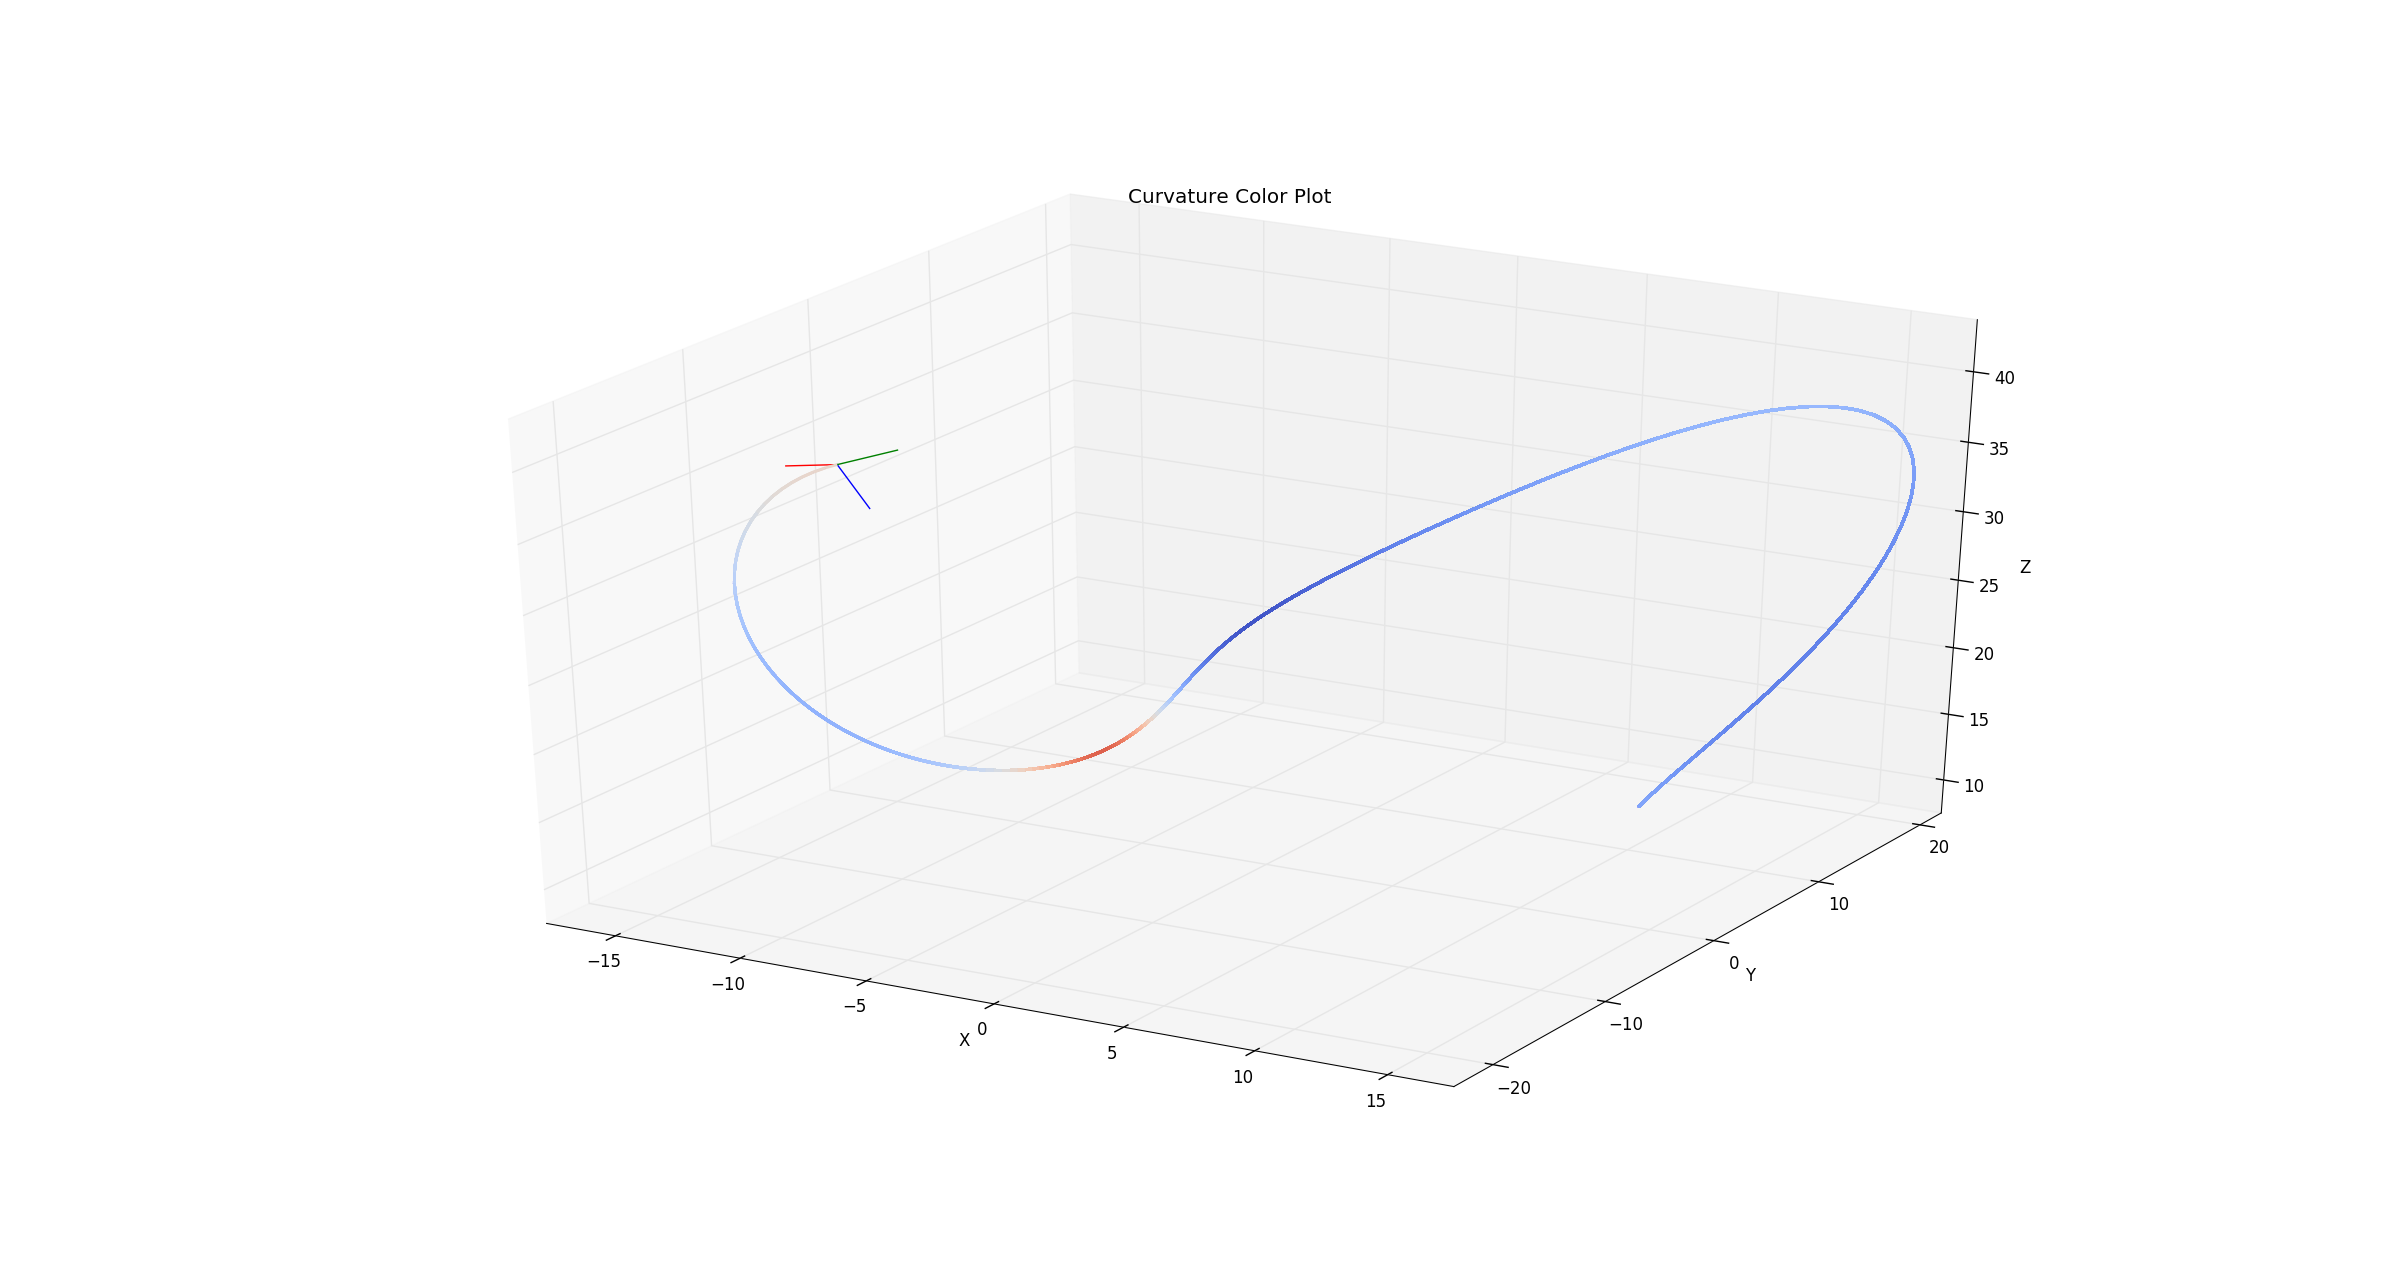
\includegraphics[width=\linewidth]{2c}
 \caption{Curvature Animation few seconds later.}
  \label{mult4}
\end{figure}
as for other solutions involving different values for $\rho$, $\sigma$ and $\beta$, check out figure \ref{ex1} and \ref{ex2}
\begin{figure}
 \centering
 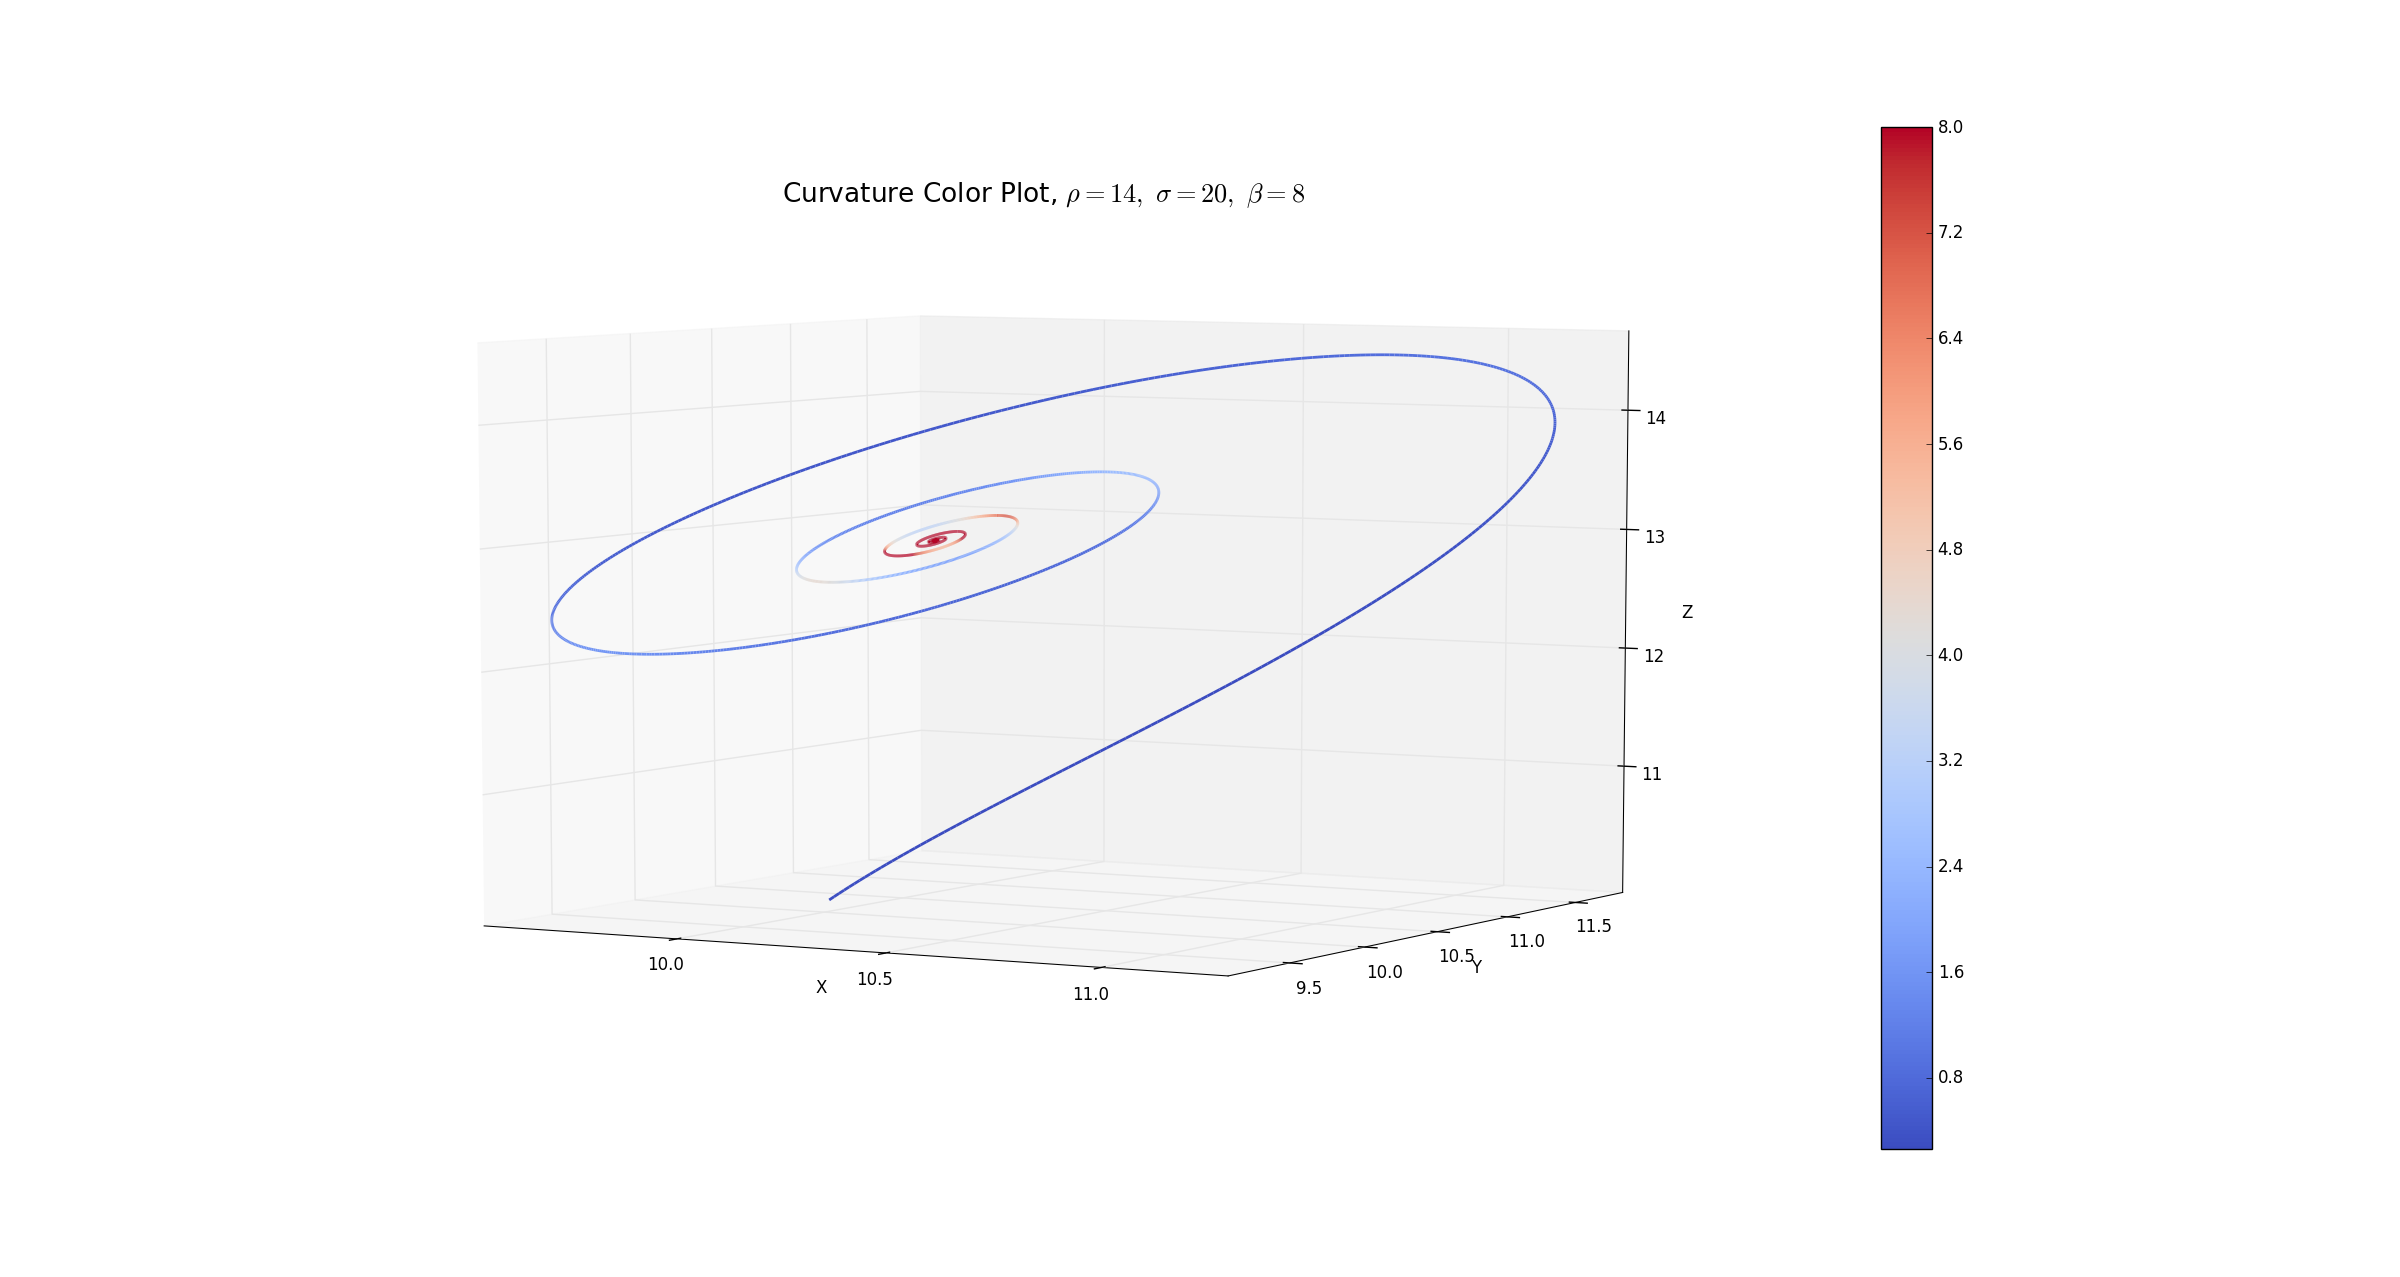
\includegraphics[width=\linewidth]{ex1}
 \caption{Curvature plot for an alternative solution which seems to converge.}
  \label{ex1}  
\end{figure}

\begin{figure}
 \centering
 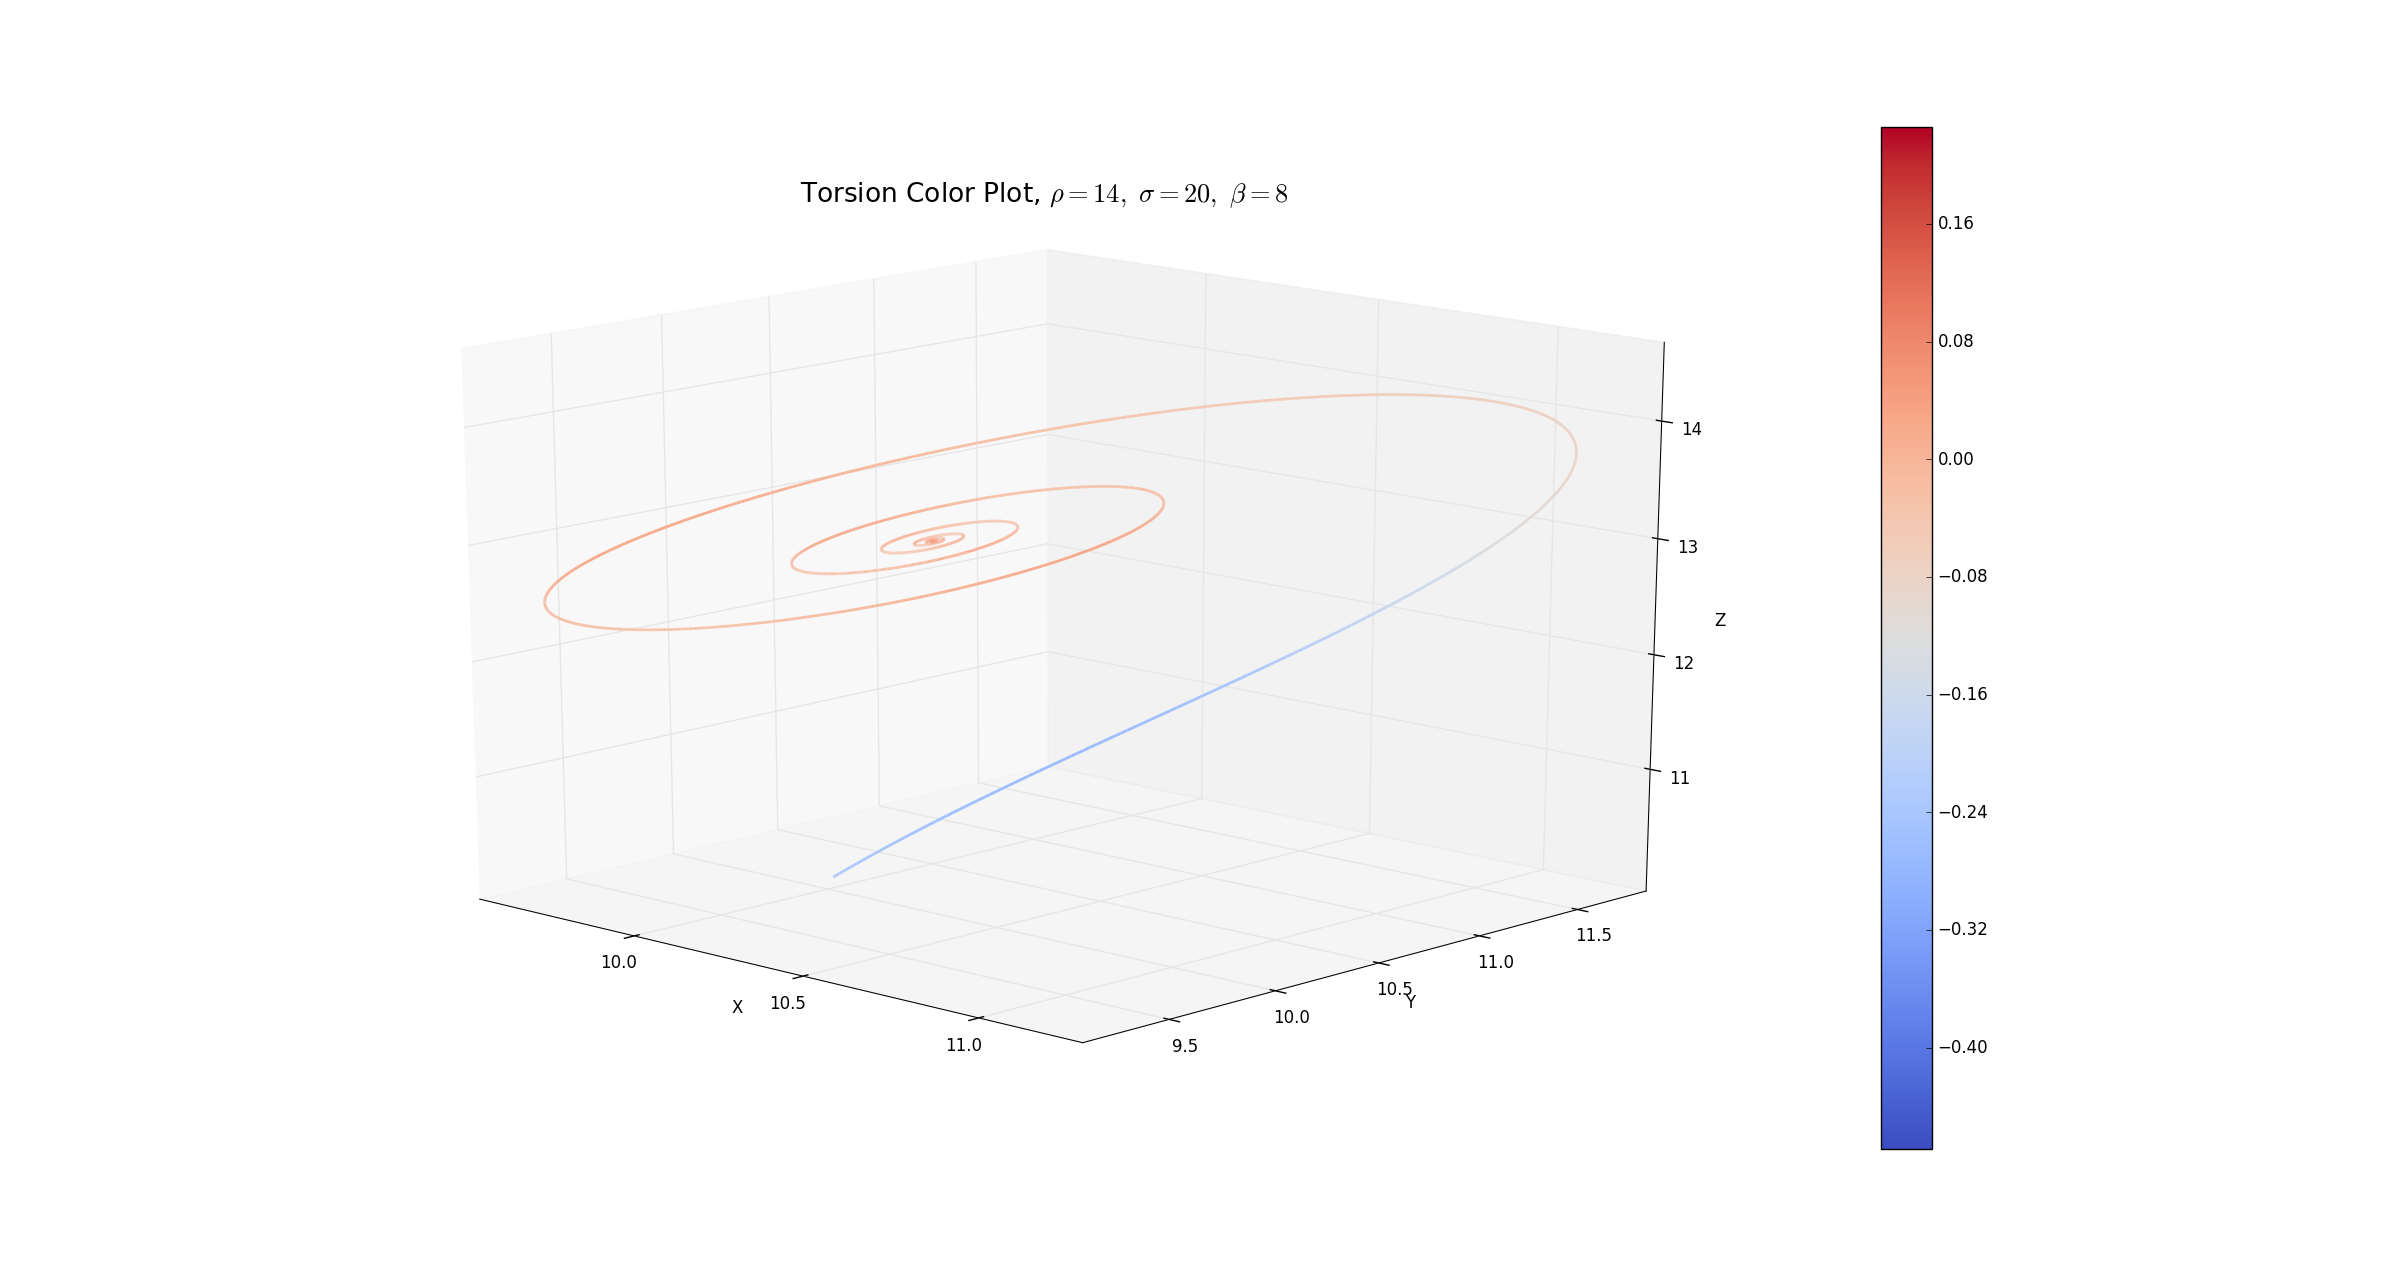
\includegraphics[width=\linewidth]{ex2}
 \caption{Torsion plot, quite homogenous.}
  \label{ex2}
\end{figure}


\section*{Task C}

\end{document}
